% !TEX program = xelatex
\documentclass[14pt, a4paper]{extreport}

%% Шрифты и язык
\usepackage{fontspec}
\setmainfont{Times New Roman}
\usepackage{polyglossia}
\setmainlanguage{russian}
\setotherlanguage{english}
% TODO: дописать про LSTM
%% Поля страницы
\usepackage[
  a4paper,
  top=2cm,
  bottom=2cm,
  left=3cm,
  right=1.5cm
]{geometry}

%% Межстрочный интервал 1.5
\usepackage{setspace}
\onehalfspacing

%% Отступ первой строки абзаца
\usepackage{indentfirst}
\setlength{\parindent}{1.25cm}

%% Заголовки глав и разделов
\usepackage{titlesec}
\titleformat{\chapter}[block]
  {\normalfont\large\bfseries\centering}
  {\chaptername\ \thechapter.}{0.5em}{}
\titlespacing*{\chapter}{0pt}{0pt}{12pt}

\titleformat{\section}
  {\normalfont\normalsize\bfseries}
  {\thesection}{0.5em}{}
\titlespacing*{\section}{0pt}{12pt}{6pt}

%% Содержание
\usepackage{tocloft}
\renewcommand{\cftchapleader}{\cftdotfill{\cftdotsep}}
\setlength{\cftbeforechapskip}{4pt}

%% Графика и таблицы
\usepackage{graphicx}
\usepackage{booktabs}
\usepackage{array}
\usepackage{longtable}
\graphicspath{{images/}}

%% Математика
\usepackage{amsmath, amssymb}

%% Листинги кода
\usepackage{listings}
\usepackage{xcolor}
\lstset{
  basicstyle=\ttfamily\small,
  breaklines=true,
  frame=single,
  numbers=left,
  numberstyle=\tiny,
  keywordstyle=\color{blue},
  commentstyle=\color{gray},
  stringstyle=\color{orange}
}

%% Гиперссылки
\usepackage[hidelinks]{hyperref}

%% Нумерация страниц — снизу по центру
\usepackage{fancyhdr}
\pagestyle{fancy}
\fancyhf{}
\fancyfoot[C]{\thepage}
\renewcommand{\headrulewidth}{0pt}

%% Библиография
\usepackage[
  backend=biber,
  style=gost-numeric,
  sorting=none
]{biblatex}
\addbibresource{bibliography.bib}

% -------------------------------------------------------
\begin{document}

%% Титульный лист
%\begin{titlepage}
\begin{center}

\textbf{МИНИСТЕРСТВО ТРАНСПОРТА РЕСПУБЛИКИ УЗБЕКИСТАН}

\vspace{0.3cm}
\textbf{ТАШКЕНТСКИЙ ГОСУДАРСТВЕННЫЙ ТРАНСПОРТНЫЙ УНИВЕРСИТЕТ}

\vspace{0.3cm}
Кафедра: \underline{\hspace{6cm}}

\vfill

{\large\bfseries ВЫПУСКНАЯ КВАЛИФИКАЦИОННАЯ РАБОТА}

\vspace{0.5cm}
{\large\bfseries на тему:}

\vspace{0.3cm}
{\large «Прогнозирование финансовых временных рядов с применением методов машинного обучения»}

\vfill

\begin{flushright}
\begin{tabular}{ll}
Выполнил(а): & \underline{\hspace{5cm}} \\[6pt]
             & (ФИО студента) \\[12pt]
Направление: & \underline{\hspace{5cm}} \\[6pt]
Группа:      & \underline{\hspace{5cm}} \\[24pt]
Научный руководитель: & \underline{\hspace{5cm}} \\[6pt]
              & (учёная степень, ФИО) \\[12pt]
Допущен(а) к защите: & \underline{\hspace{5cm}} \\[6pt]
Дата: & \underline{\hspace{5cm}} \\
\end{tabular}
\end{flushright}

\vfill

{\large Ташкент --- \the\year}

\end{center}
\end{titlepage}
\setcounter{page}{2}


%% Содержание
\tableofcontents
\newpage

%% Введение
\chapter*{Введение}
\addcontentsline{toc}{chapter}{Введение}

\textbf{Актуальность темы.}
% TODO: написать про актуальность

\textbf{Цель работы.}
% TODO: сформулировать цель

\textbf{Задачи работы:}
\begin{enumerate}
  \item % TODO
  \item % TODO
  \item % TODO
\end{enumerate}

\textbf{Объект исследования.}
% TODO

\textbf{Предмет исследования.}
% TODO

\textbf{Методы исследования.}
% TODO

\textbf{Структура работы.}
Работа состоит из введения, трёх глав, заключения, списка литературы и приложений.


%% Глава 1
\chapter{Теоретические основы прогнозирования финансовых временных рядов}

\section{Особенности финансовых временных рядов}
Временным рядом (или рядом динамики) называется последовательность значений некоторого статистического показателя (случайной величины), упорядоченных в хронологическом порядке — в последовательные моменты или периоды времени. В экономике и финансах типичными примерами временных рядов выступают курсы обмена валют, котировки акций, уровень инфляции, показатели спроса и валовой национальный продукт. В зависимости от характера фиксации времени ряды могут быть дискретными и непрерывными. В непрерывных рядах значения переменной фиксируются непрерывно во времени, однако на практике (особенно в финансах) чаще всего анализируются дискретные временные ряды, где наблюдения производятся через определенные фиксированные интервалы времени (например, ежечасно, ежедневно, ежемесячно). Таким образом, временной ряд в контексте данной работы — это упорядоченная во времени последовательность исторических значений валютного курса.

В классическом анализе любой экономический временной ряд традиционно рассматривается как результат взаимодействия нескольких основных компонент:
\begin{itemize}
    \item Тренд (тенденция) — плавно меняющаяся компонента, описывающая чистое влияние долговременных факторов и отражающая общую (вековую) тенденцию процесса к росту или снижению.
    \item Сезонность — регулярные колебания, отражающие внутригодовую или внутримесячную повторяемость экономических процессов.
    \item Цикличность — последовательность волнообразных флуктуаций (экономических циклов), длительность которых обычно превышает один год (например, циклы деловой активности).
    \item Случайная (нерегулярная) составляющая (шум) — непредсказуемые колебания, отражающие влияние множества не поддающихся учету случайных факторов.
\end{itemize}


Ключевым свойством, необходимым для анализа и моделирования, является стационарность временного ряда. Строго стационарным называется ряд, совместное распределение вероятностей которого не изменяется при сдвиге во времени. В практических исследованиях чаще опираются на понятие слабой стационарности: ряд считается стационарным, если его математическое ожидание (среднее значение) и дисперсия остаются постоянными во времени, а ковариация зависит только от временного лага.

Стационарность крайне важна, поскольку большинство классических статистических методов и теорем опираются на предположение о неизменности свойств процесса. Проблема заключается в том, что реальные финансовые ряды практически всегда нестационарны. Их среднее значение и дисперсия меняются с течением времени, формируя стохастические тренды. Для приведения таких рядов к стационарному виду обычно применяются математические преобразования, чаще всего — переход от абсолютных значений к их разностям (приращениям).

Финансовые временные ряды, в частности курсы валют, обладают ярко выраженной спецификой, которая значительно усложняет их математическое описание:
\begin{itemize}
    \item Волатильность. Для финансовых рынков характерны резкие скачки и нестабильность дисперсии. Широко известен эффект «кластеризации волатильности»: периоды сильных и резких колебаний цены часто сменяются периодами относительного затишья.
    \item Нестационарность. Валютные курсы подвержены влиянию макроэкономических трендов и структурных изменений. Часто их поведение близко к процессу «случайного блуждания» (random walk), что делает их непредсказуемыми на больших горизонтах.
    \item Автокорреляция. Текущие значения финансовых показателей и их волатильность часто зависят от прошлых значений (наличие "памяти" у рынка), что фиксируется с помощью автокорреляционных функций.
    \item Нелинейность. Динамика финансовых рынков характеризуется высокой сложностью, а поведение участников рынка приводит к тому, что изменения цен не описываются простыми линейными формулами.
    \item Шум и случайность. Финансовые показатели содержат значительную долю шума (соотношение сигнал/шум крайне низкое). На них ежеминутно влияют поступление новых случайных новостей, макроэкономическая статистика и политические события.
\end{itemize} 

Специфические свойства финансовых временных рядов порождают серьезные трудности при их прогнозировании. Из-за беспрецедентно высокой неопределенности, динамизма и хаотичности финансовой среды предсказание курсов валют является задачей повышенной сложности. Традиционные статистические подходы и линейные модели (такие как ARIMA или экспоненциальное сглаживание), несмотря на их полезность, не всегда справляются с нелинейной природой и высокой зашумленностью финансовых данных. Это обуславливает необходимость использования более сложных и гибких аналитических инструментов.

Финансовые временные ряды представляют собой сложные, хаотичные и нестационарные структуры. Присущие им специфические свойства — высокая волатильность, нелинейность, подверженность случайным шокам и структурным сдвигам — требуют для анализа и точного прогнозирования применения современных продвинутых методов, в том числе алгоритмов машинного обучения и нейронных сетей.

\section{Классические модели прогнозирования курса валют}
% TODO

\section{Методы машинного обучения в прогнозировании}
% TODO

\section{Нейросетевые модели прогнозирования}
% TODO


%% Глава 2
\chapter{Методология исследования и описание данных}

\section{Выбор объекта исследования}
% TODO

\section{Очистка и подготовка данных}
% TODO

\section{Постановка задачи прогнозирования}
% TODO

\section{Используемые модели}
% TODO


%% Глава 3
\chapter{Практическая реализация (эксперименты и результаты)}

\section{Результаты обучений классических моделей}
Для построения базового статистического прогноза временного ряда валютного курса была использована модель ARIMA. Данный подход традиционно применяется в эконометрике в качестве классического метода анализа временных рядов. В рамках данного исследования он используется как базовая модель (benchmark) для последующего объективного сравнения с более сложными алгоритмами машинного обучения и современными нейросетевыми архитектурами глубокого обучения.

Для определения оптимальной конфигурации модели использовался автоматизированный подбор параметров на основе минимизации информационного критерия Акаике (AIC). Данный критерий является эффективным инструментом, так как он представляет собой компромисс между качеством подгонки модели к историческим данным и ее сложностью («экономией»), налагая штраф за избыточное число параметров. В результате была выбрана модель ARIMA(4,1,2), показавшая наилучшее качество (минимальное значение AIC) среди рассмотренных вариантов.

Фрагмент вывода результатов подбора параметров:
\begin{lstlisting}
   ARIMA(4,1,2)(0,0,0)[0] intercept   : AIC=21290.552, Time=1.97 sec 
\end{lstlisting}
 

Обучение модели выполнялось на обучающей выборке временного ряда с использованием библиотеки statsmodels языка программирования Python. Алгоритм осуществляет оценку параметров авторегрессии и скользящего среднего, минимизируя среднеквадратичную ошибку на тренировочных данных.
\begin{lstlisting}
    from statsmodels.tsa.arima.model import ARIMA
        # Обучаем_модель_ на_ текущей _истории
    model     = ARIMA(history, order=best_order)
    model_fit = model.fit()
\end{lstlisting}

После завершения обучения модели был построен прогноз значений валютного курса на тестовой выборке. Для повышения реалистичности прогнозирования в работе использовался подход rolling forecast (скользящего прогнозирования). В отличие от прямого многошагового прогнозирования, при котором модель строит прогноз сразу на весь тестовый интервал, rolling forecast (или метод скользящего окна с переоценкой) предполагает последовательное выполнение одношаговых прогнозов.

На каждом шаге модель обучалась на текущем наборе доступных данных, после чего выполнялся прогноз только на один следующий момент времени. Затем фактическое (реальное) значение добавлялось в обучающую историю, и процедура повторялась снова. Такой подход позволяет модели постоянно адаптироваться к изменяющейся динамике временного ряда, усваивать свежие рыночные шоки и обеспечивает более высокую точность краткосрочного прогнозирования.

Для оценки качества прогнозирования использовались метрики MAE, RMSE и MAPE. Средняя абсолютная ошибка (MAE) и корень из среднеквадратичной ошибки (RMSE) измеряют абсолютные отклонения прогноза, при этом RMSE сильнее «штрафует» модель за крупные выбросы. Средняя абсолютная ошибка в процентах (MAPE) позволяет оценить точность в безразмерных (относительных) величинах, что упрощает экономическую интерпретацию. Для всех перечисленных метрик действует правило: чем меньше полученное значение, тем выше точность прогноза и лучше работает модель.
Полученные результаты оценки классической модели представлены в таблице 3.1.

\begin{table}[h!]
\centering
\caption{Результаты оценки точности модели ARIMA}
\begin{tabular}{|l|c|}
\hline
\textbf{Метрика} & \textbf{Значение} \\ \hline
MAE  & 19.05 сум \\ \hline
RMSE & 28.55 сум \\ \hline
MAPE & 0.15\% \\ \hline
\end{tabular}
\end{table}

Для наглядной оценки поведения алгоритма полученные прогнозные значения были наложены на фактический график тестовой выборки валютного курса.
\begin{figure}[h!]
    \centering
    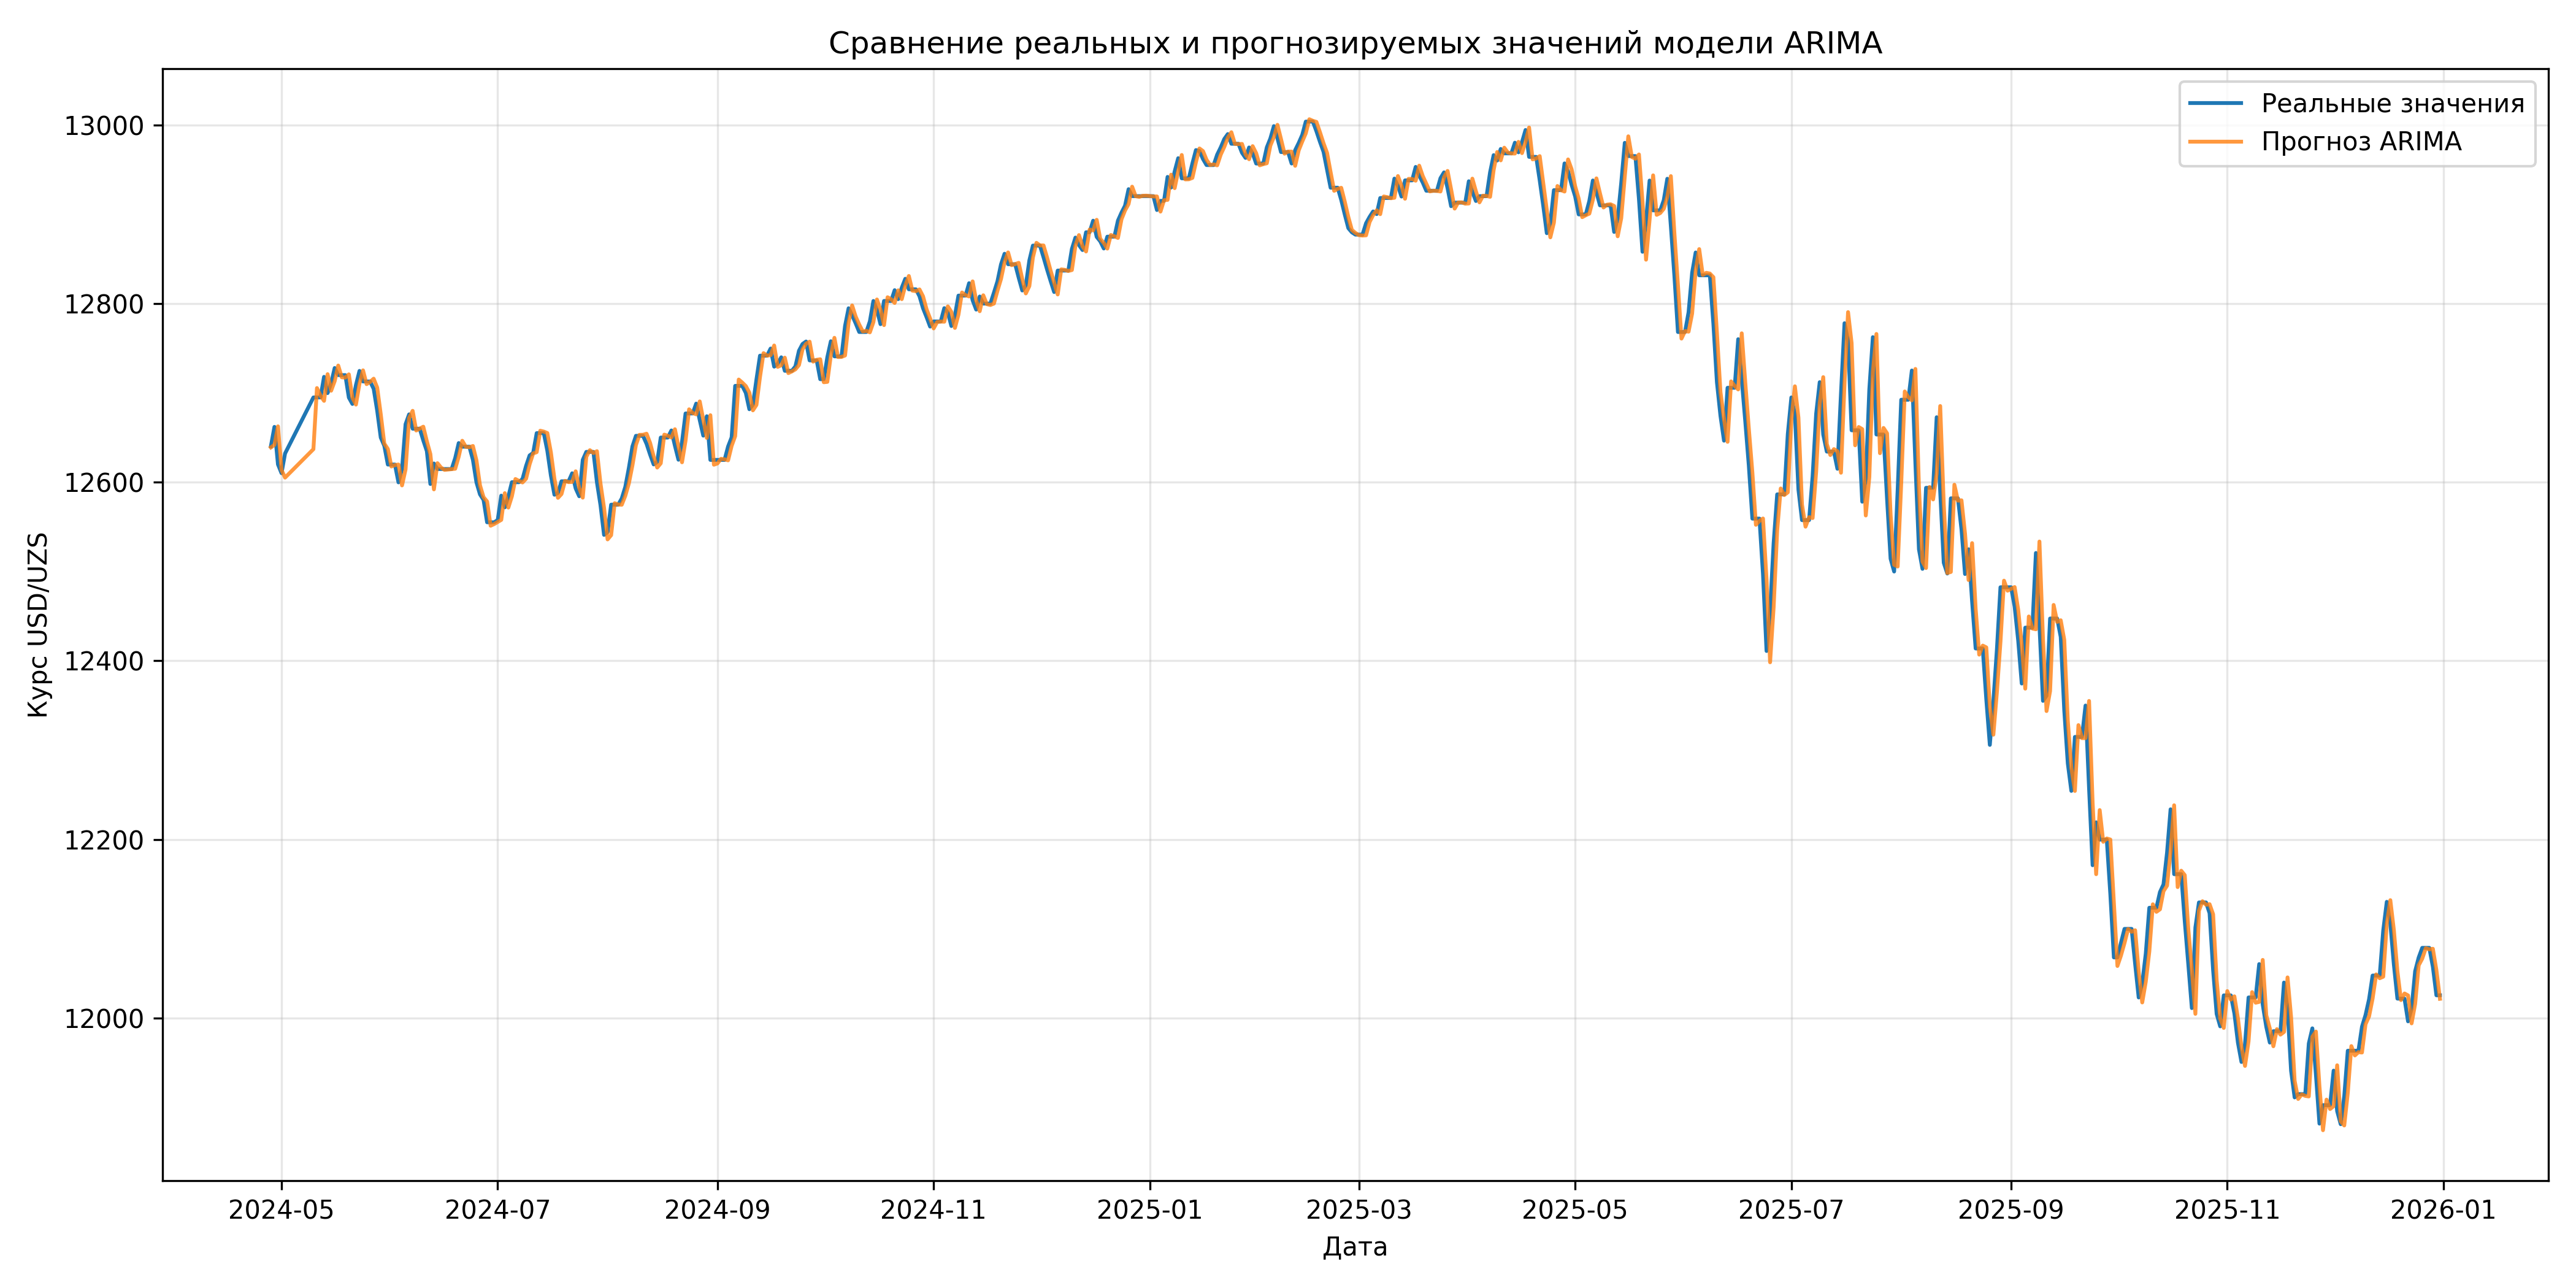
\includegraphics[width=0.9\textwidth]{python/collect-usd-rates/plots/arima_forecast.png}
    \caption{Сравнение реальных и прогнозируемых значений модели ARIMA}
    \label{fig:arima_forecast}
\end{figure}
Рисунок 3.1 – Сравнение реальных и прогнозируемых значений модели ARIMA

На рисунке видно, что модель ARIMA достаточно хорошо воспроизводит общую динамику временного ряда и корректно улавливает долгосрочный восходящий тренд изменения курса. При этом в отдельных участках наблюдаются отклонения прогноза от реальных значений, особенно в периоды повышенной волатильности, где классическая линейная модель склонна к излишнему сглаживанию локальных ценовых пиков.

Модель ARIMA с использованием подхода rolling forecast демонстрирует высокую степень совпадения прогнозируемых и реальных значений временного ряда. Модель успешно воспроизводит общую динамику изменения валютного курса и корректно реагирует на локальные колебания ряда благодаря механизму постоянного обновления истории. Полученные значения метрик (MAPE = 0.15\%) свидетельствуют о высоком качестве краткосрочного прогнозирования. Тем не менее, заметное сглаживание пиковых скачков указывает на фундаментальные ограничения линейного статистического подхода в условиях резкой волатильности, что подтверждает целесообразность исследования более сложных нейросетевых архитектур.

\section{Результаты ML-моделей}
Для исследования возможностей методов машинного обучения в задаче прогнозирования валютного курса была использована модель Random Forest. Данный алгоритм выбран как один из наиболее распространенных ансамблевых методов регрессии, способный выявлять нелинейные зависимости между признаками и целевой переменной.

В отличие от модели ARIMA, алгоритм Random Forest не учитывает временную структуру данных напрямую. Поэтому для обучения модели были сформированы лаговые признаки, представляющие собой значения валютного курса за предыдущие периоды времени.

В базовой конфигурации модели использовались семь лаговых признаков, соответствующих значениям курса за семь предыдущих дней. Дополнительно был проведен эксперимент с использованием тридцати лаговых признаков. Однако увеличение количества признаков не привело к улучшению качества прогнозирования и сопровождалось ростом значений ошибок. Это связано с тем, что добавление избыточного количества лагов может вносить дополнительный информационный шум и декоррелировать работу деревьев в ансамбле неоптимальным образом. 
\begin{table}[h!]
\centering
\caption{Результаты оценки точности модели Random Forest с 30 лагами}
\begin{tabular}{|l|c|}
\hline
\textbf{Метрика} & \textbf{Значение} \\ \hline
MAE  & 133.97 сум \\ \hline
RMSE & 164.83 сум \\ \hline
MAPE & 1.05\% \\ \hline
\end{tabular}
\end{table}

\begin{figure}[h!]
    \centering
    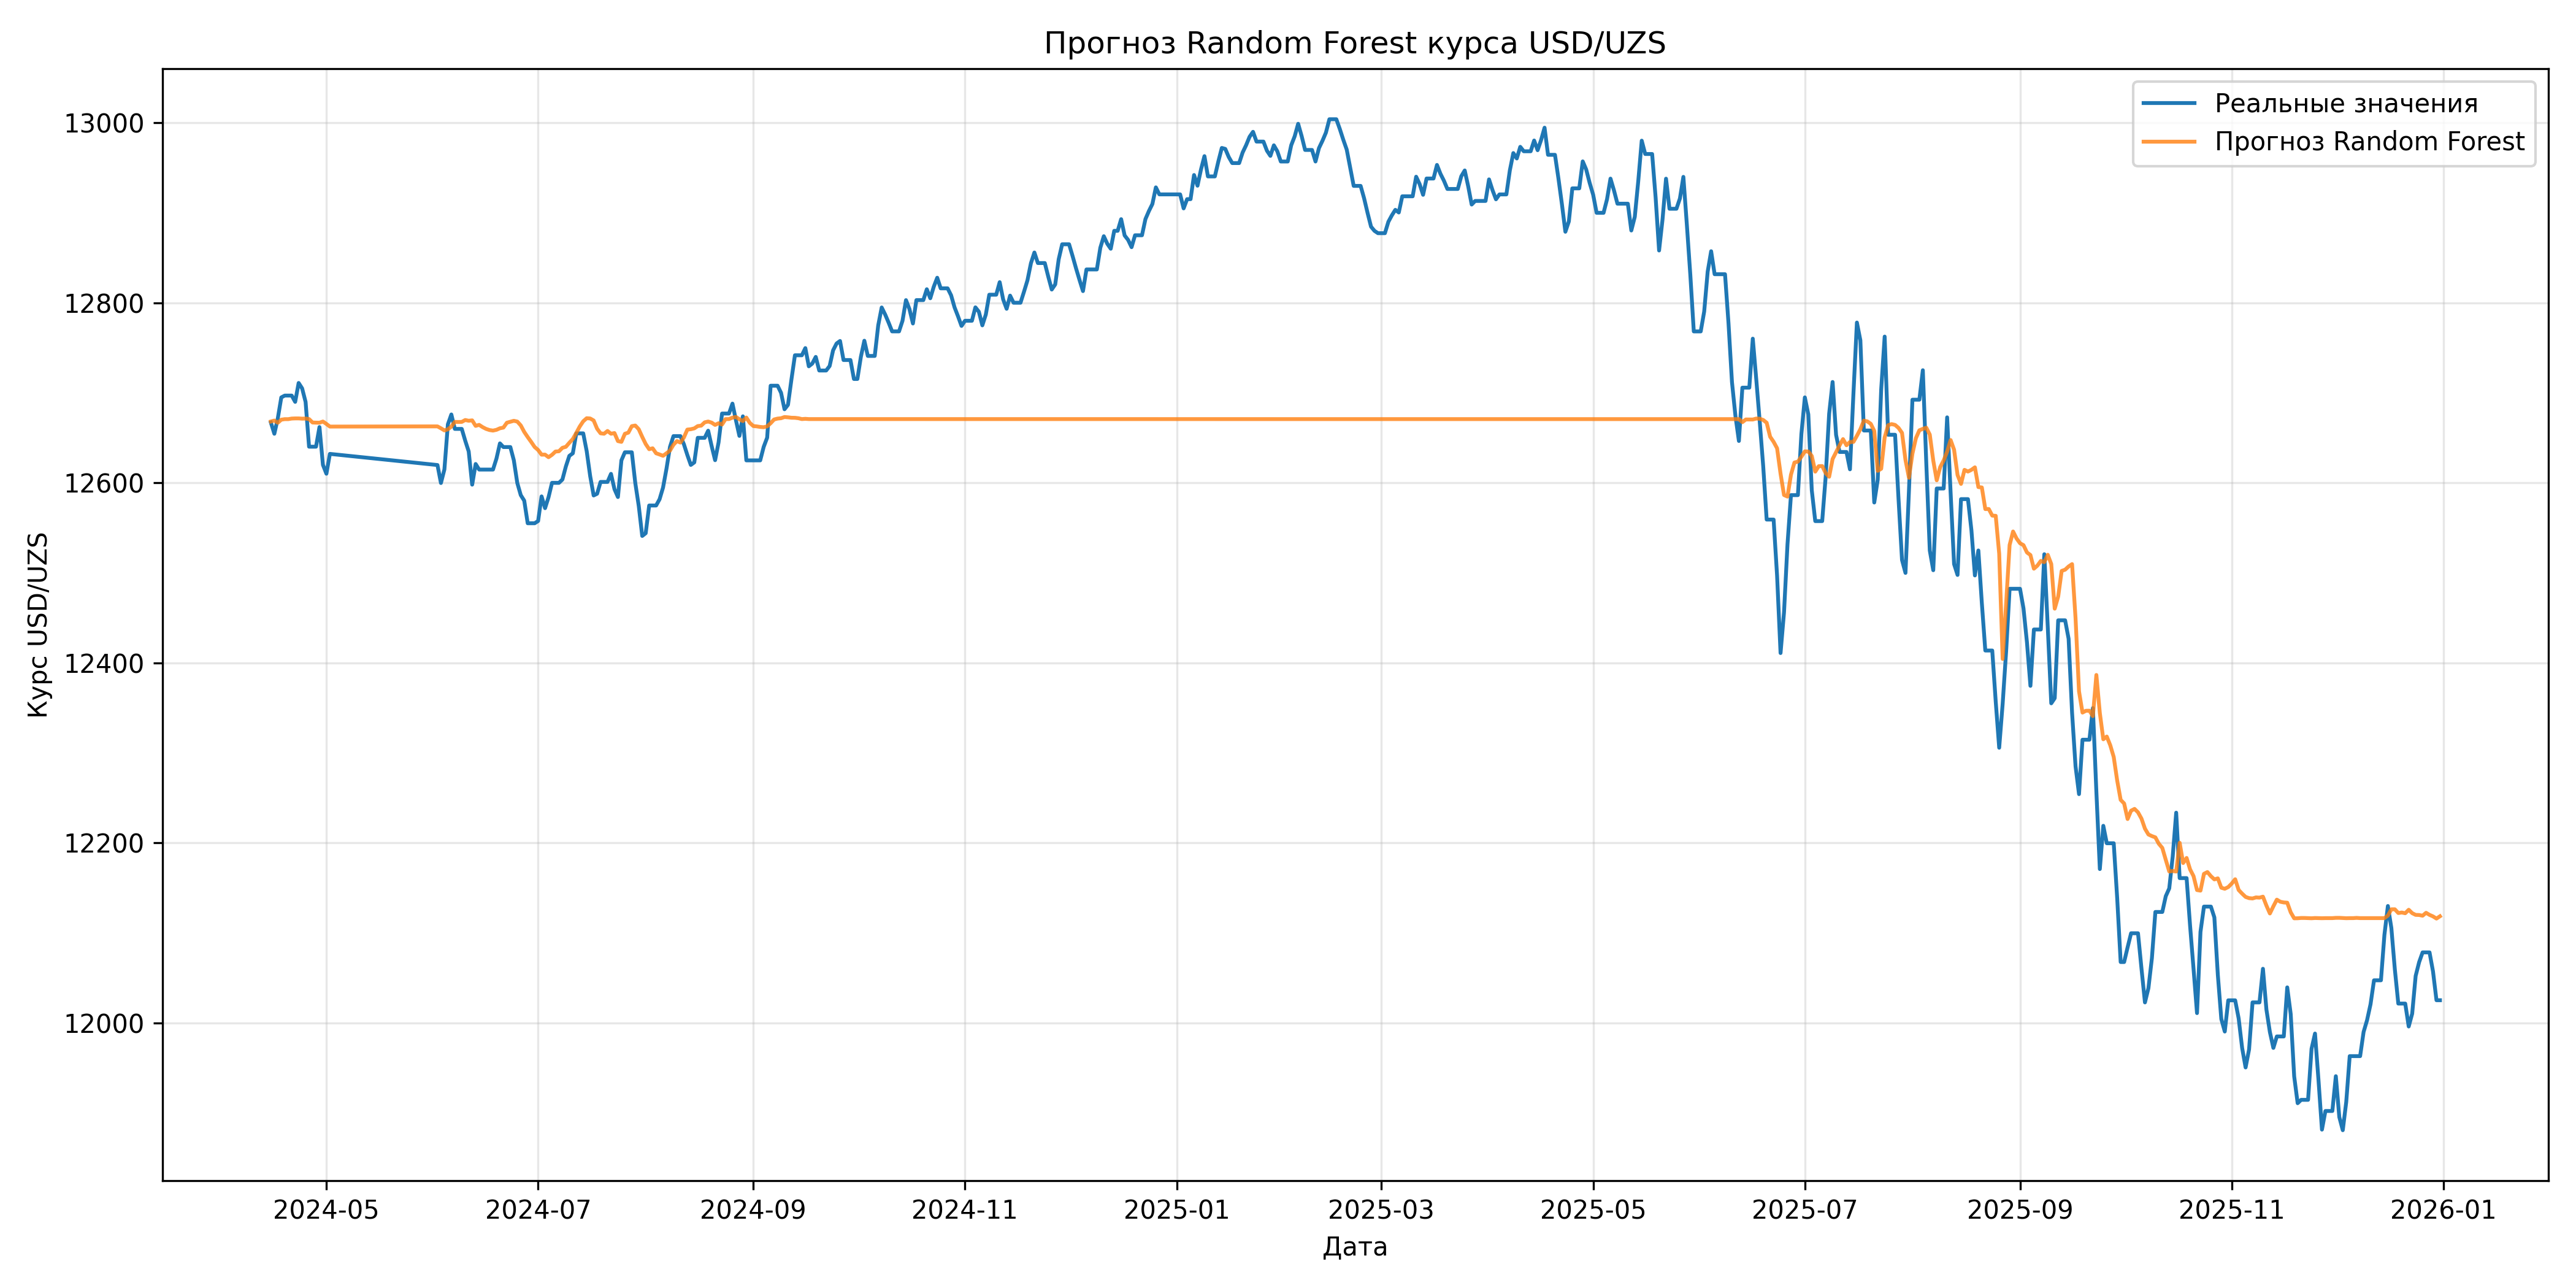
\includegraphics[width=0.9\textwidth]{python/collect-usd-rates/plots/rf_forecastTEST30lag.png}
    \caption{Сравнение реальных и прогнозируемых значений модели Random Forest(30 лагов)}
    \label{fig:rf_forecast30}
\end{figure}

Поэтому для дальнейшего анализа была выбрана конфигурация с семью лагами.

Обучение модели выполнялось на обучающей выборке с использованием библиотеки Scikit-Learn языка программирования Python. Для построения ансамбля использовалось 100 деревьев решений. Суть метода заключается в том, что каждое дерево независимо обучается на случайной подвыборке, а итоговый результат усредняется, что позволяет существенно снизить общую дисперсию модели и избежать переобучения.
Инициализация модели в программной среде имеет следующий вид:
\begin{lstlisting}
from sklearn.ensemble import RandomForestRegressor

model = RandomForestRegressor(
    n_estimators=100,
    random_state=42
)
\end{lstlisting}

После завершения обучения модель была применена к тестовой выборке для получения прогнозных значений валютного курса. В ходе данного этапа на вход обученному алгоритму подавались векторы сформированных лаговых признаков, на основе которых формировался точечный одношаговый прогноз.

Для количественной оценки качества прогнозирования использовались метрики MAE, RMSE и MAPE. Полученные результаты представлены в таблице 3.3.

\begin{table}[h!]
\centering
\caption{Результаты оценки точности модели Random Forest с 7 лагами}
\begin{tabular}{|l|c|}
\hline
\textbf{Метрика} & \textbf{Значение} \\ \hline
MAE  & 112.01 сум \\ \hline
RMSE & 146.64 сум \\ \hline
MAPE & 0.88\% \\ \hline
\end{tabular}
\end{table}

Для наглядной оценки поведения модели полученные прогнозные значения были наложены на фактический график тестовой выборки.
\begin{figure}[h!]
    \centering
    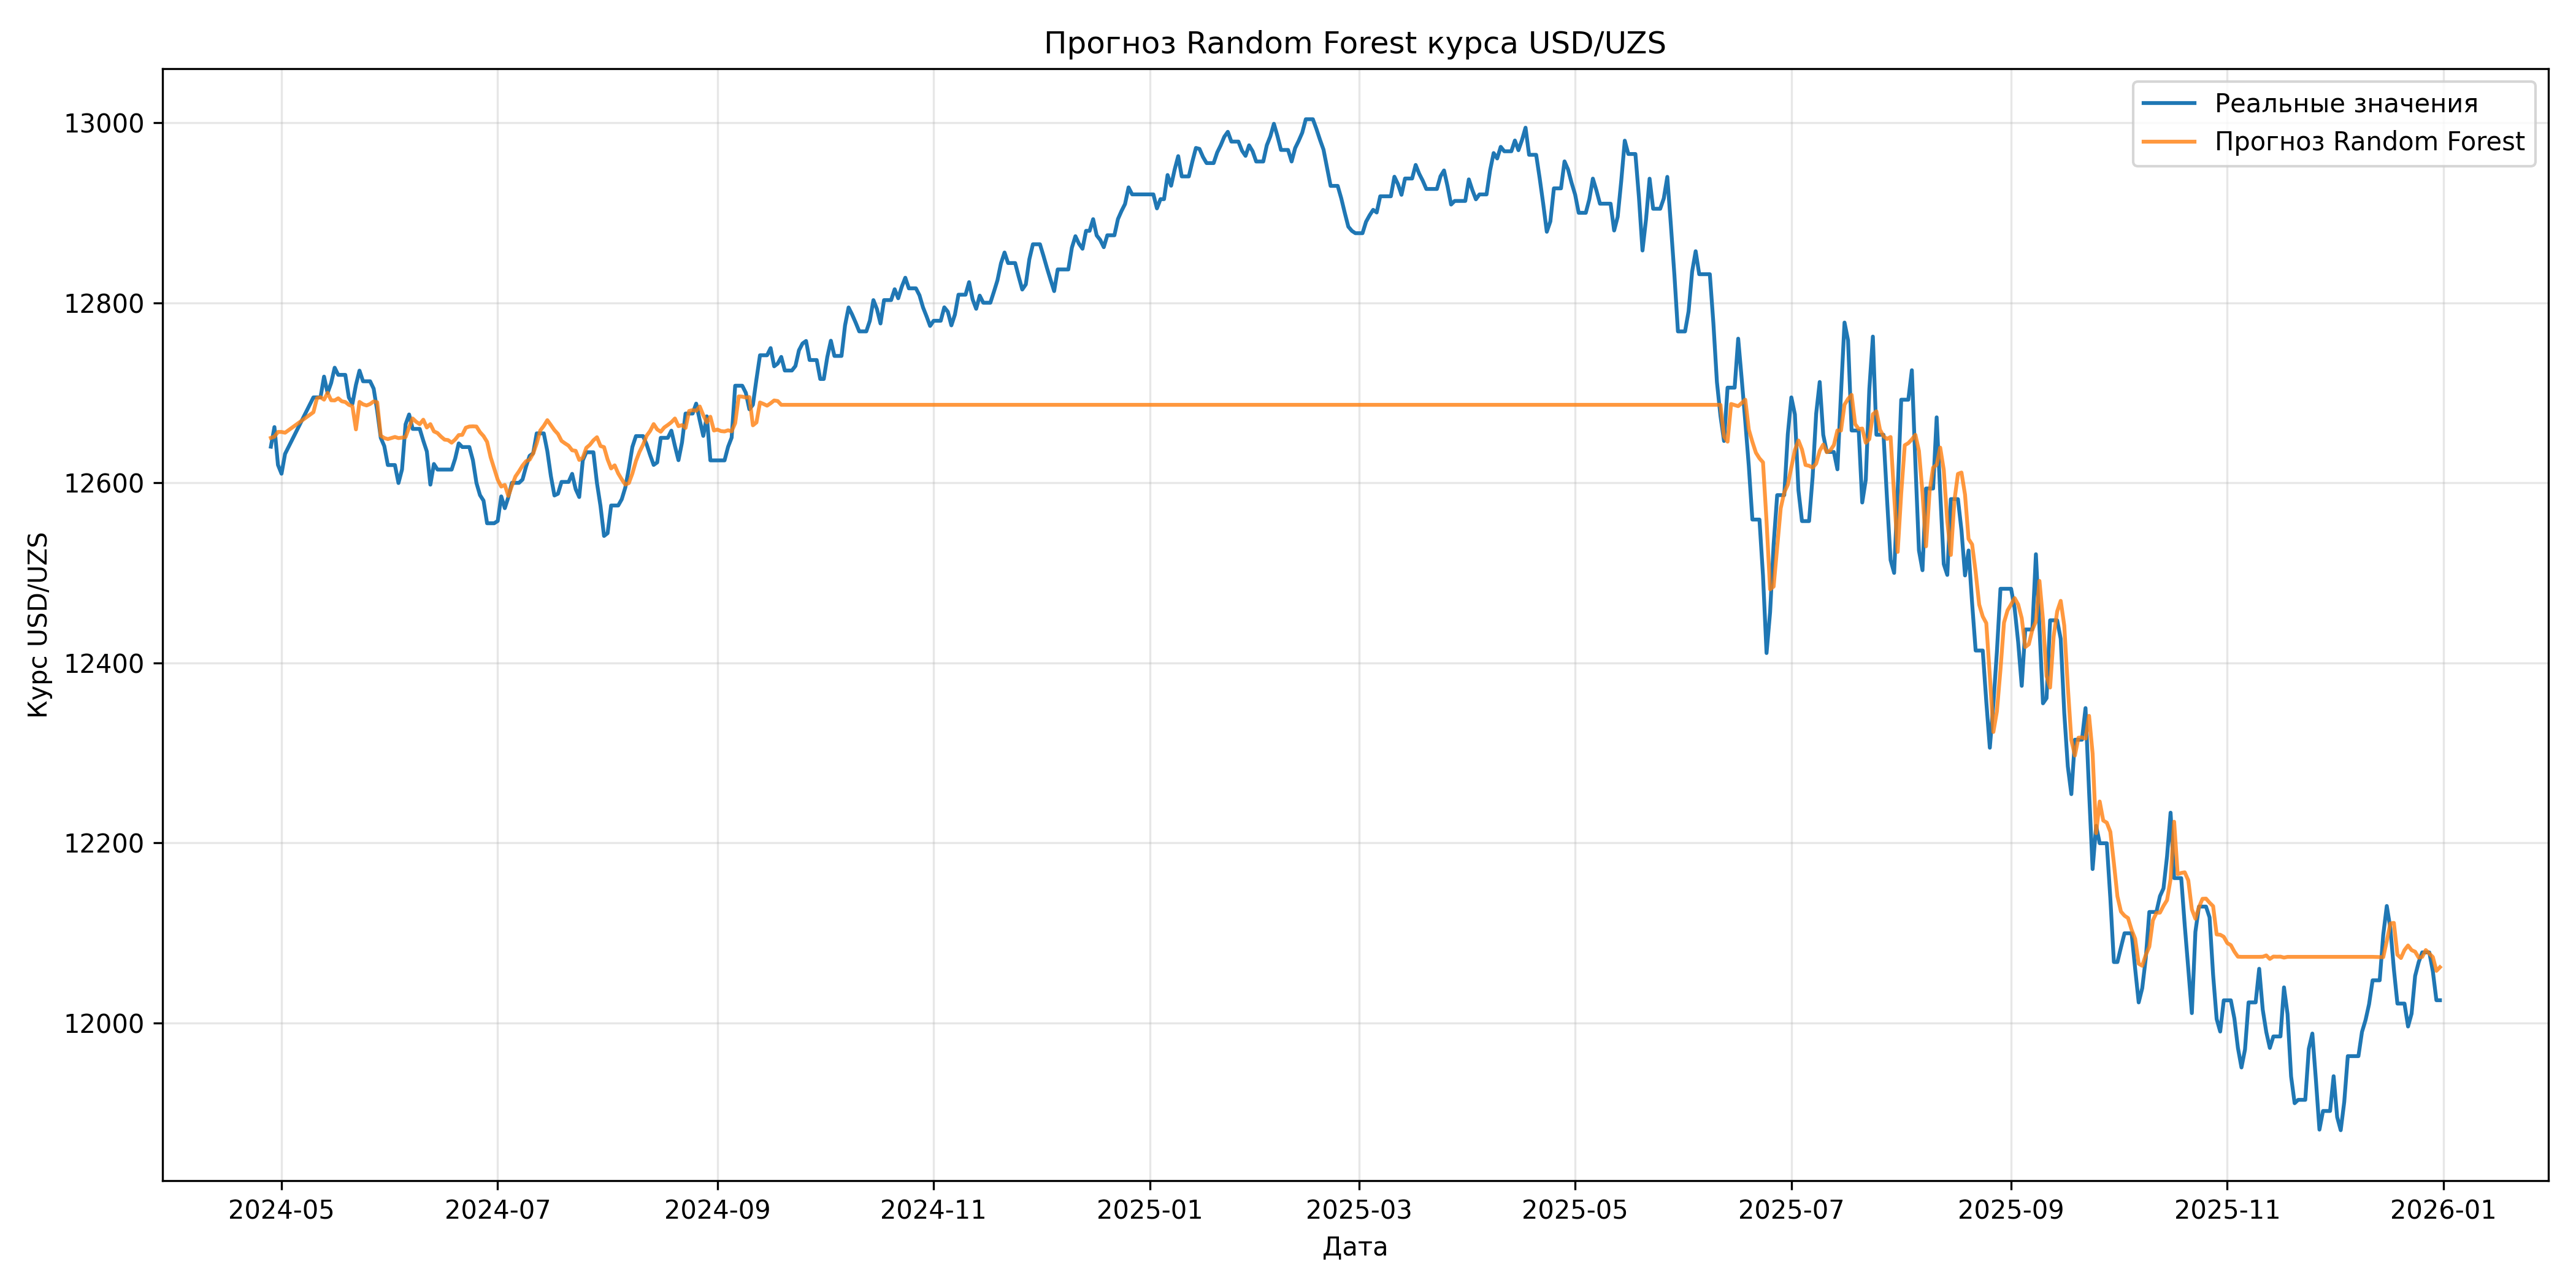
\includegraphics[width=0.9\textwidth]{python/collect-usd-rates/plots/rf_forecast.png}
    \caption{Сравнение реальных и прогнозируемых значений модели Random Forest(7 лагов)}
    \label{fig:rf_forecast7}
\end{figure}

На рисунке видно, что модель Random Forest в целом воспроизводит основные тенденции временного ряда. Вместе с тем прогноз демонстрирует склонность к сглаживанию резких изменений курса и приближению к среднему уровню ряда. На участках продолжительного тренда наблюдаются отклонения прогнозируемых значений от фактических данных. Это объясняется математической спецификой алгоритмов на основе деревьев: случайный лес осуществляет усреднение значений в терминальных узлах (листьях) и принципиально не способен экстраполировать значения, выходящие за пределы тех, на которых он обучался.

Таким образом, модель Random Forest показала способность прогнозировать общую динамику валютного курса и обеспечила приемлемое качество прогноза. Проведенный эксперимент также показал, что увеличение числа лаговых признаков с 7 до 30 не приводит к улучшению результатов. Полученные данные будут использованы на следующем этапе исследования для последующего сравнения с другими моделями прогнозирования (в частности, с рекуррентными нейронными сетями).

\section{Построение и обучение LSTM}
Нейросетевые алгоритмы, в особенности рекуррентные сети, обладают высокой чувствительностью к масштабу входных данных. Для обеспечения корректной работы алгоритмов оптимизации и ускорения сходимости весов использовался предварительно нормализованный ряд. Приведение всех значений валютного курса к единому диапазону от 0 до 1 осуществлялось с применением метода минимаксного масштабирования (MinMaxScaler). Масштабирование выполнялось строго на обучающей выборке, после чего полученные параметры преобразования применялись к тестовой выборке для исключения утечки данных.
В отличие от классических моделей и простых алгоритмов машинного обучения, архитектура LSTM принимает на вход данные в виде трехмерного тензора (образцы, временные шаги, признаки). Для учета временно́й зависимости производилось формирование последовательностей методом скользящего окна. В данной конфигурации использовалось окно длиной 10 наблюдений: для прогнозирования курса на следующий день на вход нейросети подавалась последовательность значений за 10 предыдущих дней. Такое окно позволяет алгоритму уловить краткосрочные паттерны и локальные тренды.
Разделение набора данных на обучающую (train) и тестовую (test) выборки производилось в пропорции 80/20. Разделение выполнялось строго в хронологическом порядке без перемешивания, чтобы сохранить естественную структуру временного ряда.

Для решения задачи прогнозирования использовалась рекуррентная нейронная сеть долгой краткосрочной памяти (Long Short-Term Memory, LSTM). Эта архитектура разработана специально для преодоления проблемы затухающего градиента и способна эффективно выявлять долгосрочные зависимости в последовательных данных благодаря системе внутренних шлюзов (gates).
Спроектированная архитектура сети включает один скрытый слой LSTM, состоящий из 50 нейронов. Данного количества достаточно для извлечения скрытых признаков из финансовых рядов без чрезмерного усложнения модели. За ним следует полносвязный выходной слой Dense(1) с линейной функцией активации, который агрегирует извлеченные признаки и выдает итоговое предсказанное значение валютного курса.
В качестве функции потерь (loss function) использовалась среднеквадратичная ошибка (MSE) — стандартная метрика для задач регрессии, минимизация которой позволяет обучать параметры модели. В качестве алгоритма оптимизации был выбран передовой оптимизатор Adam (Adaptive Moment Estimation), который комбинирует идеи накопления импульса и адаптивной скорости обучения для каждого параметра, что делает его крайне эффективным для обучения глубоких нейросетей.
Сводная информация по архитектуре модели и количеству обучаемых параметров (model.summary()) представлена в таблице 3.4.
\begin{table}[h!]
\centering
\caption{Архитектура модели LSTM}
\label{tab:lstm_architecture}
\begin{tabular}{|l|c|c|}
\hline
\textbf{Layer (type)} & \textbf{Output Shape} & \textbf{Param \#} \\ \hline
\texttt{lstm (LSTM)}  & (None, 50)            & 10\,400 \\ \hline
\texttt{dense (Dense)} & (None, 1)             & 51 \\ \hline
\textbf{Всего параметров:}      & \multicolumn{2}{c|}{10\,451 (40.82 КБ)} \\ \hline
\textbf{Обучаемых параметров:}  & \multicolumn{2}{c|}{10\,451 (40.82 КБ)} \\ \hline
\textbf{Необучаемых параметров:}& \multicolumn{2}{c|}{0} \\ \hline
\end{tabular}
\end{table}

Процесс обучения модели заключался в итеративной корректировке весов для минимизации функции потерь. Обучение проводилось в течение 20 эпох (\texttt{epochs=20}), что означает 20 полных проходов алгоритма по обучающему набору данных. Для обновления градиентов данные разбивались на пакеты (\texttt{batch\_size=32}), что позволяет сбалансировать скорость вычислений и стабильность сходимости.
Дополнительно в процессе обучения 10\% обучающей выборки выделялось под валидацию (\texttt{validation\_split=0.1}). Это необходимо для независимого контроля качества: после каждой эпохи вычислялась ошибка на валидационном наборе, что позволяло отслеживать потенциальное переобучение (overfitting).

\begin{figure}[h!]
    \centering
    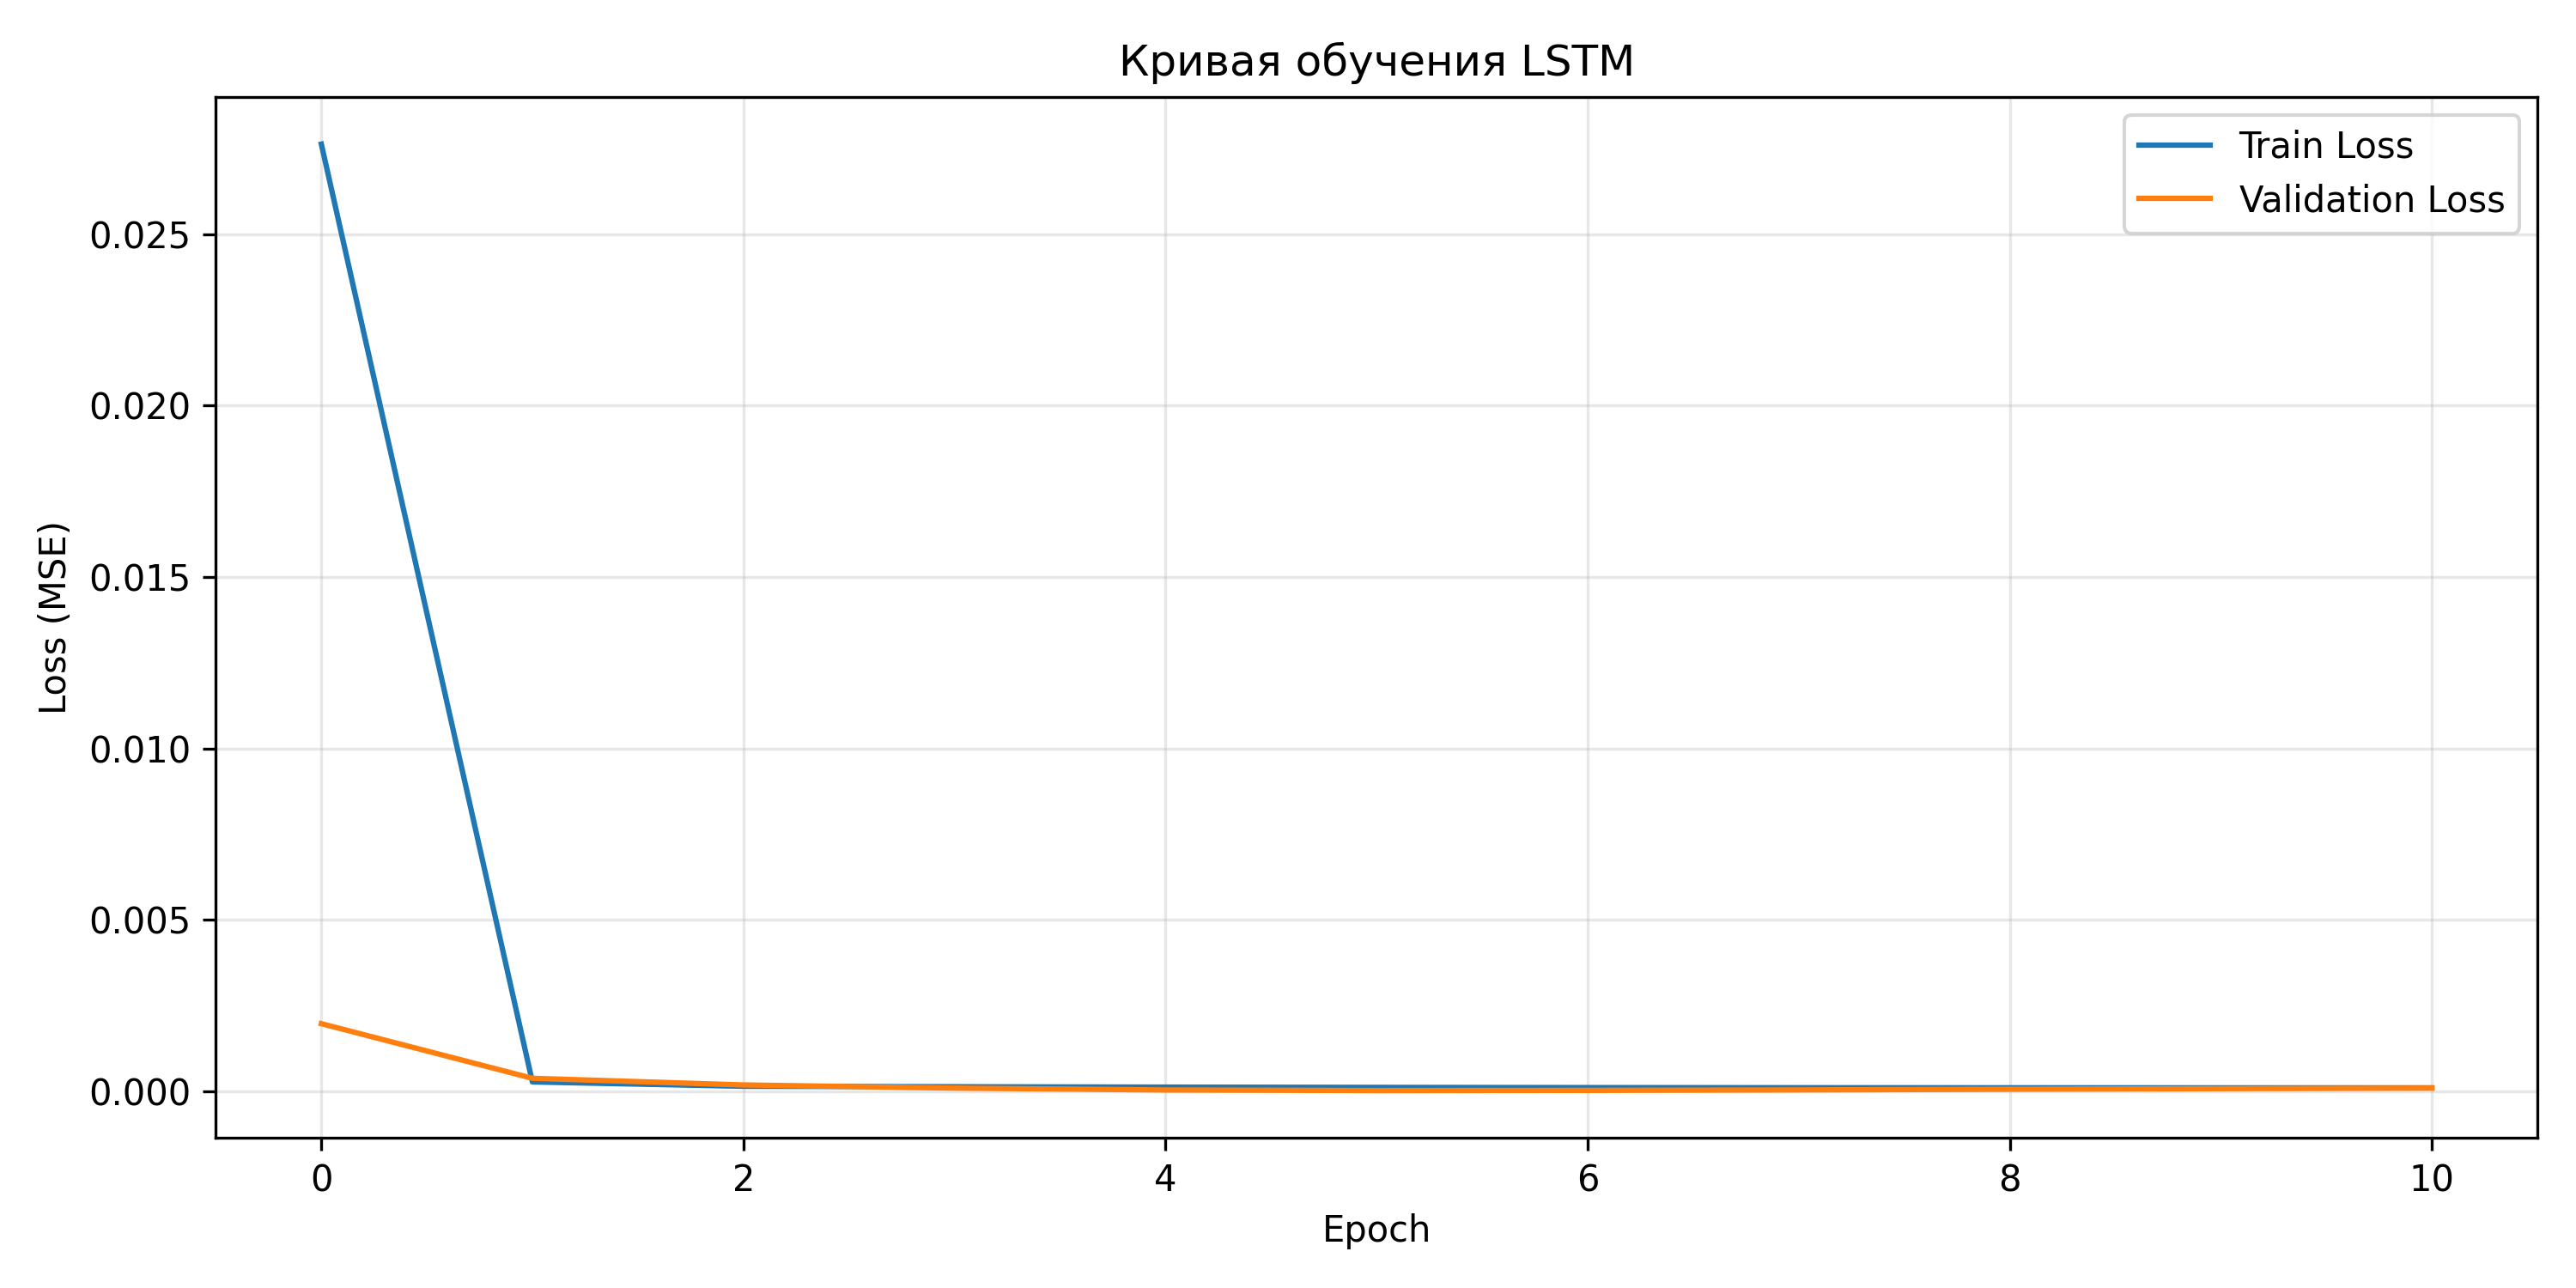
\includegraphics[width=0.9\textwidth]{python/collect-usd-rates/plots/lstm_train_graph.png}
    \caption{Динамика функции потерь (MSE) в процессе обучения модели LSTM}
    \label{fig:lstm_epochs}
\end{figure}

На рисунке видно, что значения функции потерь быстро снижаются в первые эпохи обучения и далее стабилизируются. Существенного расхождения между обучающей и валидационной ошибками не наблюдается, что свидетельствует об отсутствии выраженного переобучения модели.

После завершения процесса обучения модель была протестирована на отложенной (тестовой) выборке, которую алгоритм ранее не наблюдал. Модель получала на вход историческое окно из 10 наблюдений и формировала одношаговый прогноз.

\begin{figure}[h!]
    \centering
    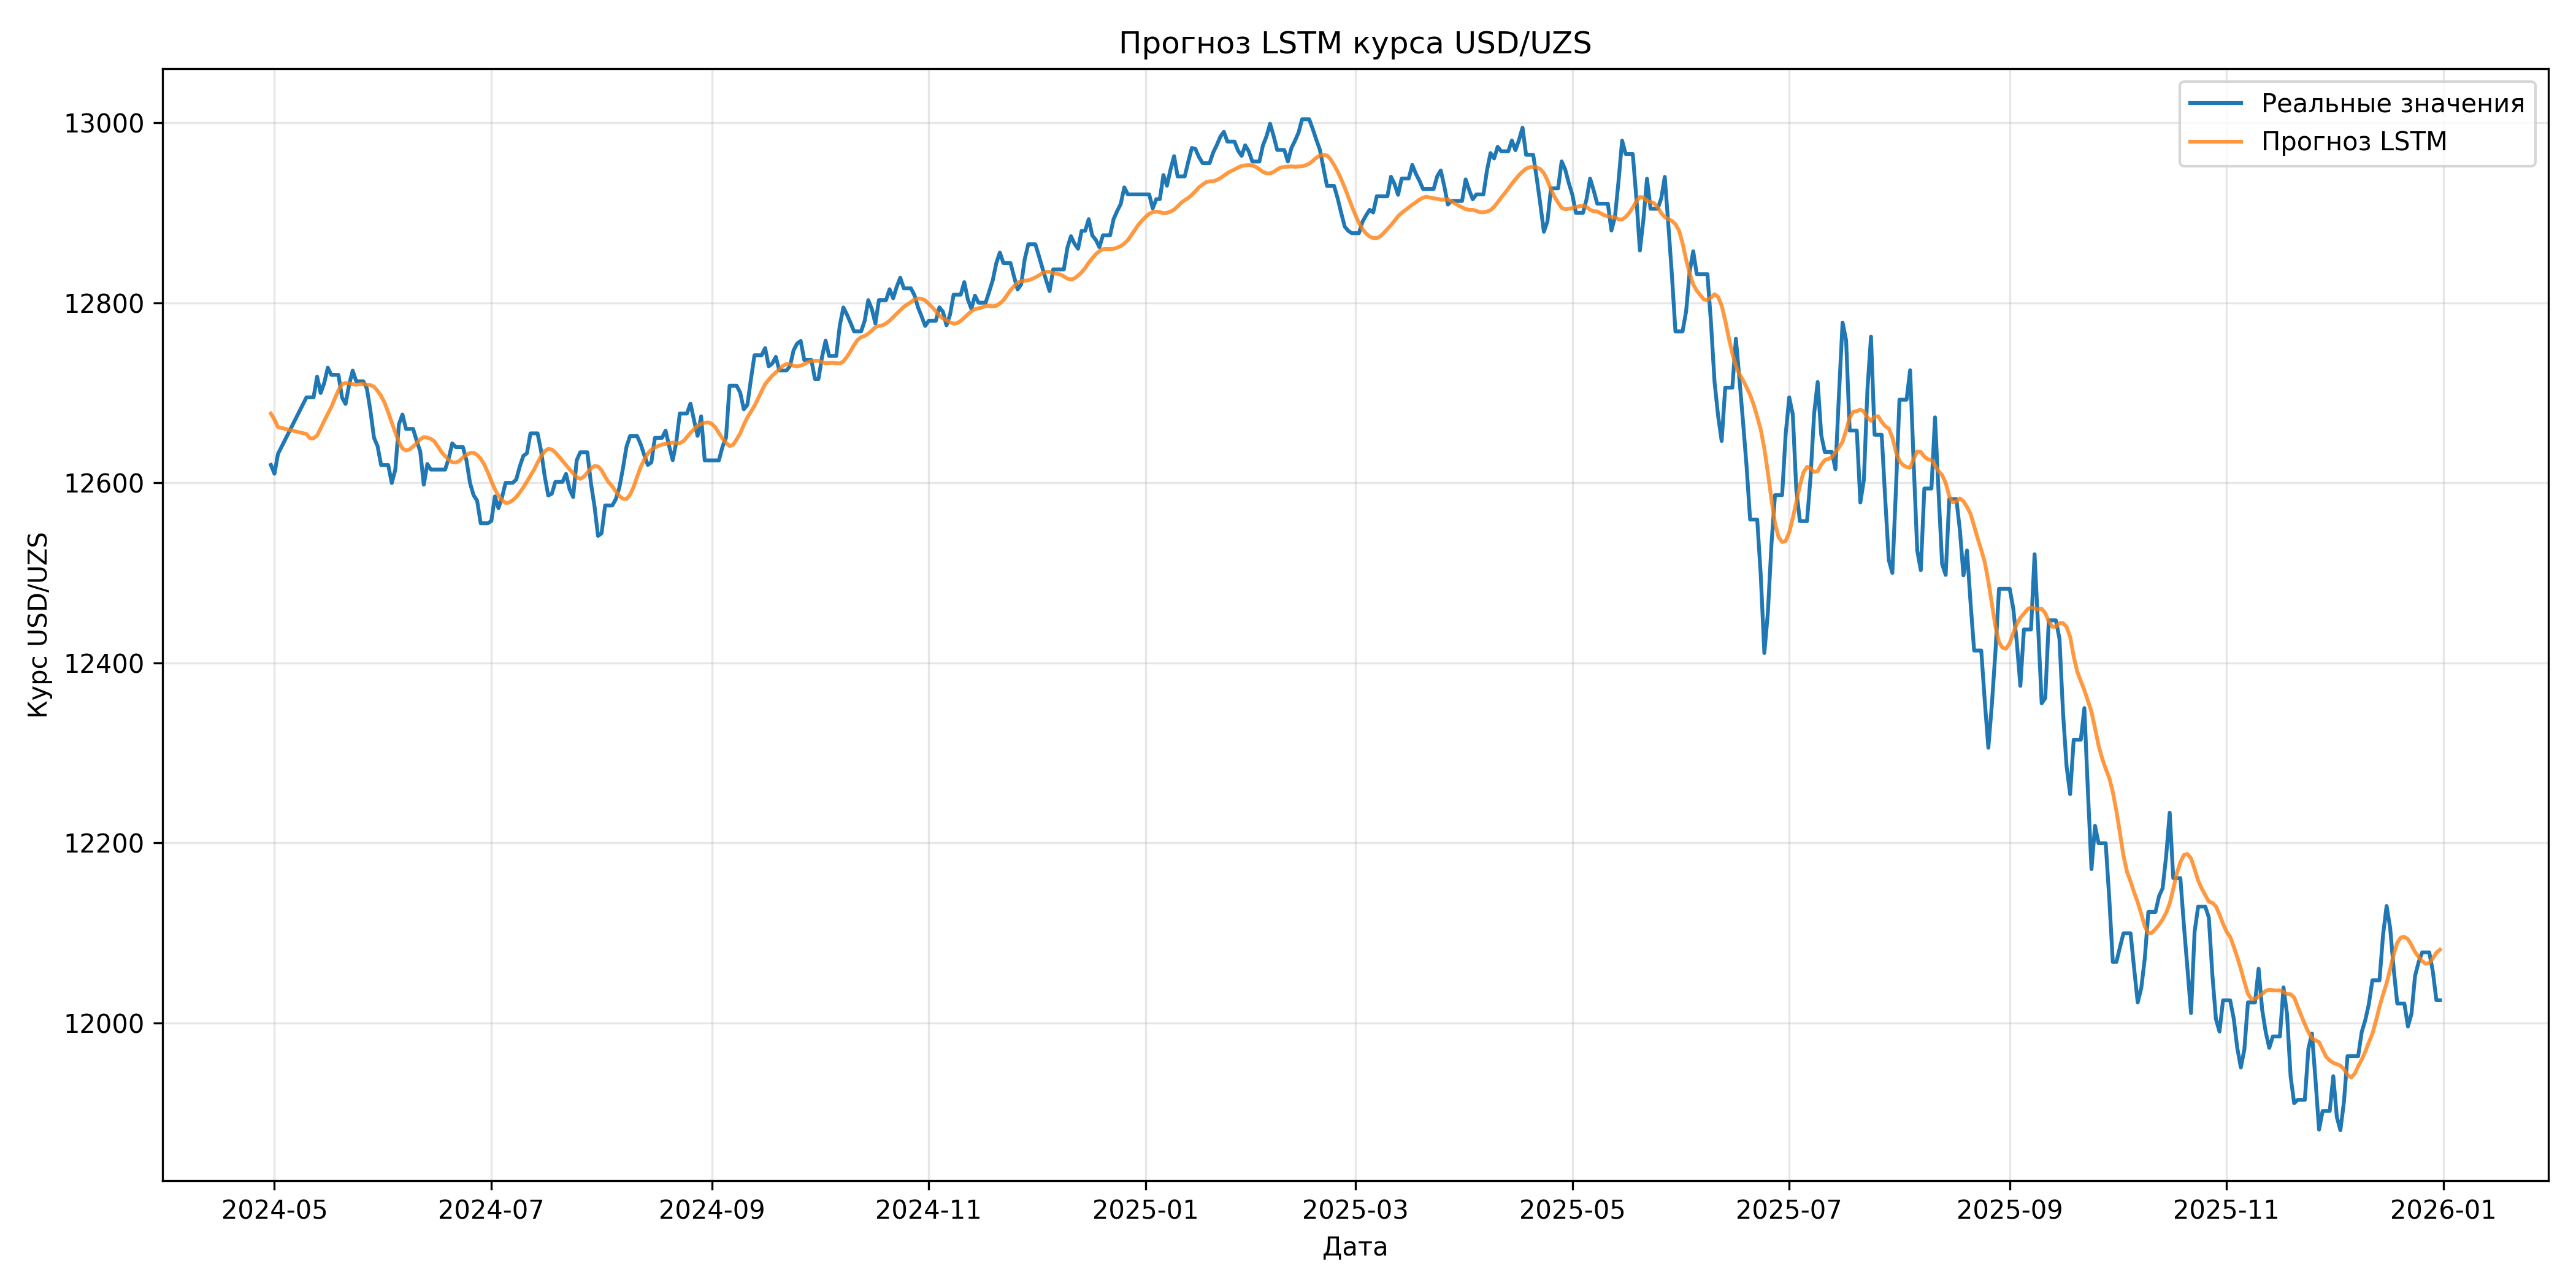
\includegraphics[width=0.9\textwidth]{python/collect-usd-rates/plots/lstm_forecast.png}
    \caption{Сравнение фактических и прогнозных значений курса USD/UZS (модель LSTM)}
    \label{fig:lstm_forecast}
\end{figure}


На рисунке представлено сравнение фактических значений курса USD/UZS и прогнозных значений, полученных с помощью модели LSTM. Модель успешно воспроизводит общий тренд временного ряда и корректно отслеживает основные изменения курса валюты. При этом наблюдается некоторое сглаживание краткосрочных колебаний, характерное для нейросетевых моделей данного типа.

Для количественной оценки качества прогнозирования были использованы показатели MAE, RMSE и MAPE. Результаты расчета метрик ошибки на тестовой выборке представлены в таблице 3.5.
\begin{table}[h!]
\centering
\caption{Метрики качества модели LSTM}
\label{tab:lstm_metrics}
\begin{tabular}{|l|c|}
\hline
\textbf{Метрика} & \textbf{Значение} \\ \hline
MAE  & 40{,}74 сум \\ \hline
RMSE & 54{,}37 сум \\ \hline
MAPE & 0{,}33\% \\ \hline
\end{tabular}
\end{table}

Полученные результаты свидетельствуют о высокой точности прогноза. Средняя относительная ошибка составила 0,33 \%, что подтверждает способность модели эффективно выявлять закономерности изменения валютного курса.

Таким образом, модель LSTM продемонстрировала высокое качество прогнозирования курса USD/UZS. Использование рекуррентной архитектуры позволило учитывать временные зависимости во входных данных и получать прогнозы, близкие к фактическим значениям. Полученные результаты будут использованы на следующем этапе исследования для сравнительного анализа с моделями ARIMA и Random Forest.

\section{Сравнение результатов всех моделей}
Для объективной оценки эффективности рассмотренных моделей было проведено количественное сравнение их предсказательной способности по метрикам средней абсолютной ошибки (MAE), корня из среднеквадратичной ошибки (RMSE) и средней абсолютной ошибки в процентах (MAPE). Сводные результаты оценки на тестовой выборке представлены в таблице 3.6.
\begin{table}[h!]
\centering
\caption{Сравнение метрик качества прогнозирования различных моделей}
\label{tab:models_comparison}
\begin{tabular}{|l|c|c|c|}
\hline
\textbf{Модель} & \textbf{MAE, сум} & \textbf{RMSE, сум} & \textbf{MAPE, \%} \\ \hline
ARIMA           & 19{,}05           & 28{,}55            & 0{,}15 \\ \hline
LSTM            & 40{,}74           & 54{,}37            & 0{,}33 \\ \hline
Random Forest   & 112{,}01          & 146{,}64           & 0{,}88 \\ \hline
\end{tabular}
\end{table}

Данные таблицы показывают, что наименьшие значения ошибок продемонстрировала классическая статистическая модель ARIMA. Средняя абсолютная ошибка для этого алгоритма составила 19,05 сумов, а средняя относительная ошибка (MAPE) — всего 0,15 \%. Нейросетевая модель LSTM также показала высокое качество прогнозирования, однако её ошибки оказались несколько выше по сравнению с эконометрическим подходом. Наибольшие значения ошибок были получены для ансамблевой модели машинного обучения Random Forest, что указывает на её меньшую приспособленность к анализу данного одномерного временного ряда без использования дополнительных экзогенных факторов.

Визуальный анализ результатов показал, что все рассматриваемые модели способны воспроизводить общий долгосрочный тренд изменения валютного курса. Однако характер формируемых прогнозов существенно различается в деталях.
Модель ARIMA наиболее точно отслеживает краткосрочные изменения и локальные шоки временного ряда благодаря использованию механизма rolling forecast (скользящего прогнозирования с постоянным переобучением). Модель LSTM успешно воспроизводит общую динамику курса и демонстрирует хорошую адаптацию к изменениям тренда, однако в отдельных участках она склонна сглаживать резкие ценовые колебания, что является характерной особенностью глубоких нейронных сетей при работе с сильно зашумленными финансовыми данными. Модель Random Forest в большей степени ориентируется на усреднённые исторические значения в терминальных узлах деревьев и значительно хуже реагирует на быстрые структурные изменения курса.
Сравнение моделей исключительно по метрикам ошибки не дает полной картины, так как каждый алгоритм обладает своими фундаментальными особенностями, определяющими границы его применимости. Основные преимущества и недостатки рассмотренных методов систематизированы в таблице 3.7.
\begin{table}[h!]
\centering
\caption{Преимущества и недостатки моделей прогнозирования}
\label{tab:models_pros_cons}
\begin{tabular}{|l|p{6.2cm}|p{6.2cm}|}
\hline
\textbf{Модель} & \textbf{Преимущества} & \textbf{Недостатки} \\ \hline
ARIMA & 
Высокая точность на коротких горизонтах, простота математической интерпретации & 
Строго требует стационарности ряда, плохо улавливает сложную нелинейность \\ \hline
Random Forest & 
Простота обучения, устойчивость к выбросам и статистическому шуму, не требует масштабирования & 
Хуже учитывает внутреннюю временную структуру, не способна экстраполировать тренд за пределы обучающей выборки \\ \hline
LSTM & 
Способна выявлять сложнейшие нелинейные зависимости и сохранять долгосрочную память о поведении ряда & 
Более высокая вычислительная сложность, требует больших объемов данных, является «черным ящиком» \\ \hline
\end{tabular}
\end{table}

Результаты исследования показывают, что выбор оптимальной модели напрямую зависит от поставленной задачи. Для одношагового краткосрочного прогнозирования валютного курса модель ARIMA продемонстрировала наилучшие результаты. В то же время, архитектура LSTM обладает несравненно более высокой гибкостью и может быть крайне перспективной для решения более сложных задач многошагового прогнозирования, особенно при добавлении дополнительных макроэкономических факторов и увеличении объемов обучающих выборок.

В рамках практической части исследования были реализованы и протестированы три принципиально различных подхода к прогнозированию курса USD/UZS: классическая статистическая модель ARIMA, алгоритм ансамблевого машинного обучения Random Forest и рекуррентная нейросетевая модель LSTM.
Сравнение результатов показало, что на рассматриваемом наборе данных наилучшее качество прогнозирования продемонстрировала модель ARIMA. Она обеспечила минимальные значения показателей MAE, RMSE и MAPE, что однозначно свидетельствует о ее высокой точности в задачах краткосрочного прогноза при использовании механизма скользящего окна.
Модель LSTM также показала высокую эффективность и обеспечила результаты, близкие к модели ARIMA. При этом данная нейросетевая архитектура обладает значительным потенциалом для дальнейшего развития и применения в более сложных многомерных задачах прогнозирования финансовых рынков.
Модель Random Forest уступила двум другим подходам по всем используемым метрикам качества. Несмотря на свою фундаментальную способность выявлять нелинейные зависимости, данный алгоритм оказался менее эффективным для анализа строго упорядоченного одномерного временного ряда валютного курса без конструирования дополнительных сложных признаков.
Таким образом, для задачи одношагового прогнозирования курса USD/UZS на основе исключительно исторических значений временного ряда наиболее точной и эффективной моделью в рамках проведённого исследования оказалась ARIMA.


\section{Интерпретация результатов}
Полученные количественные результаты показали убедительное преимущество классической статистической модели ARIMA над алгоритмом Random Forest и нейросетевой архитектурой LSTM. Это может быть связано со специфическими особенностями исследуемого временного ряда. После проведения либерализации валютного рынка в 2017 году курс USD/UZS демонстрировал выраженный и относительно устойчивый девальвационный тренд с умеренной стохастической волатильностью. В подобных условиях линейные статистические модели, специально разработанные для работы со стационарными (или приводимыми к стационарности) рядами, способны предельно эффективно выявлять существующие закономерности. В ситуации стабильного тренда избыточная сложность алгоритмов машинного обучения не требуется, а классические параметрические методы обеспечивают наименьшую ошибку предсказания без необходимости использования сложных нелинейных алгоритмов.

Сложность прогнозирования финансовых показателей заключается в том, что валютный курс определяется не только собственной историей изменения (авторегрессионной «памятью» рынка), но и масштабным влиянием макроэкономических факторов: уровня инфляции, процентных ставок, состояния платежного баланса страны, прямых действий Центрального банка и общей внешнеэкономической конъюнктуры.

В настоящем исследовании применялся подход «чисто временного ряда», при котором для моделирования использовались исключительно исторические значения самого курса. Это накладывает определённые ограничения на предельную точность прогнозирования, так как внешние макроэкономические шоки способны вызывать резкие структурные сдвиги в динамике, которые невозможно предсказать исключительно на основе прошлых котировок. Понимание этого ограничения является важным аспектом при оценке реальной эффективности любых одномерных прогностических алгоритмов.

Несмотря на указанные ограничения, полученные результаты могут быть успешно использованы для краткосрочного прогнозирования валютного курса, а также служить надежной количественной основой для принятия управленческих решений в финансовой и банковской сфере (например, при хеджировании валютных рисков или планировании экспортно-импортных операций). Наибольший практический интерес для внедрения представляет модель ARIMA, показавшая на данной выборке наилучшее соотношение между высокой точностью одношагового прогноза, математической прозрачностью и относительной сложностью реализации.

Проведённое исследование статистически подтвердило возможность применения методов анализа временных рядов для прогнозирования курса USD/UZS. Все рассмотренные математические классы моделей продемонстрировали способность корректно воспроизводить общую динамику валютного курса.
Наиболее точный и адекватный краткосрочный прогноз был получен с использованием статистической модели ARIMA. Модель долгой краткосрочной памяти (LSTM) также показала высокое качество прогнозирования. Учитывая способность таких нейросетевых архитектур учитывать сложные нелинейные зависимости, LSTM может рассматриваться как крайне перспективное направление дальнейших исследований — в частности, при переходе к многомерному анализу и включению в модель дополнительных макроэкономических факторов. Использование ансамблевого метода Random Forest оказалось менее эффективным в рамках узкой задачи анализа одномерного финансового ряда.


%% Заключение
\chapter*{Заключение}
\addcontentsline{toc}{chapter}{Заключение}

Выпускная квалификационная работа была посвящена исследованию и сравнительному анализу методов прогнозирования валютного курса USD/UZS на основе классических моделей временных рядов, алгоритмов машинного обучения и современных нейросетевых архитектур.

Актуальность выбранной темы обусловлена высокой практической значимостью прогнозирования валютных курсов для финансовых организаций, предприятий внешнеэкономической деятельности, государственных структур и частных инвесторов. В условиях нестабильности финансовой среды и мировой экономики возрастает острая потребность в инструментах, позволяющих получать максимально точные и обоснованные прогнозы изменения котировок.

На этапе теоретического исследования были систематизированы основы анализа финансовых временных рядов, а также проведено математическое обоснование применения традиционных статистических методов прогнозирования, алгоритмов машинного обучения и рекуррентных нейросетевых моделей. Особое внимание было уделено специфике валютного курса как сложного экономического показателя, который характеризуется нестационарностью, высоким уровнем информационного шума и поведением, близким к случайному блужданию.

В рамках практической реализации в качестве объекта исследования был выбран официальный курс доллара США к узбекскому суму (USD/UZS). Для проведения корректного анализа использовались исторические данные исключительно за период после либерализации валютного рынка Республики Узбекистан (начиная с сентября 2017 года), что позволило исключить нерыночные структурные сдвиги. На этапе подготовки данных были выполнены все необходимые методологические процедуры: очистка временного ряда, нормализация значений и формирование лаговых признаков для обучения моделей.

В ходе эксперимента были программно реализованы и протестированы четыре конфигурации прогнозирования: статистическая модель ARIMA в двух режимах (rolling forecast с переобучением и статический прогноз без переобучения), алгоритм ансамблевого машинного обучения Random Forest и рекуррентная нейросетевая модель долгой краткосрочной памяти (LSTM). Для объективной оценки качества прогнозирования применялся комплекс стандартных статистических метрик: средняя абсолютная ошибка (MAE), среднеквадратичная ошибка (MSE), корень из среднеквадратичной ошибки (RMSE) и средняя абсолютная ошибка в процентах (MAPE).

Основные результаты исследования показали, что все рассмотренные модели способны воспроизводить общую динамику изменения валютного курса. Наименьшие абсолютные ошибки были получены для модели ARIMA с rolling forecast (MAPE = 0,15\%), однако данный подход использует механизм постоянного переобучения, что даёт методологическое преимущество перед моделями с однократным обучением. При корректном сравнении в равных условиях (без переобучения) наилучшие результаты продемонстрировала нейросетевая модель LSTM (MAPE = 0,33\%), значительно превзошедшая как Random Forest (MAPE = 0,88\%), так и статическую ARIMA (MAPE = 1,89\%).

Проведённое исследование позволяет сделать два ключевых вывода. Во-первых, для оперативного краткосрочного прогнозирования с возможностью постоянного обновления модели наиболее эффективна ARIMA с rolling forecast. Во-вторых, при необходимости автономного прогнозирования без переобучения нейросетевая модель LSTM демонстрирует значительное превосходство над классическими методами.

Практическая значимость работы заключается в возможности использования полученных результатов и построенных моделей для краткосрочного прогнозирования валютных курсов. Предложенные алгоритмы могут применяться при разработке аналитических систем поддержки принятия решений в банковской и финансовой сфере.

Перспективы дальнейших исследований связаны с переходом к многомерному анализу, включением дополнительных макроэкономических факторов (инфляции, процентных ставок, платежного баланса), применением более сложных нейросетевых архитектур и использованием моделей ARCH/GARCH для более точного учёта волатильности финансовых рынков.

Цель выпускной квалификационной работы достигнута, а поставленные задачи выполнены в полном объёме.

%% Список литературы
\printbibliography[title={Список литературы}]
\addcontentsline{toc}{chapter}{Список литературы}

%% Приложения
\chapter*{Приложения}
\addcontentsline{toc}{chapter}{Приложения}
\renewcommand{\thesection}{\Asbuk{section}}
\setcounter{section}{0}

\section{Приложение А. Код модели LSTM}
\label{app:lstm}

\begin{lstlisting}[language=Python, basicstyle=\small\ttfamily, breaklines=true]
import pandas as pd
import numpy as np
import matplotlib.pyplot as plt
import random
import os
import warnings

import tensorflow as tf
from tensorflow.keras.models import Sequential
from tensorflow.keras.layers import LSTM, Dense
from tensorflow.keras.callbacks import EarlyStopping
from sklearn.preprocessing import MinMaxScaler
from sklearn.metrics import mean_absolute_error, mean_squared_error

warnings.filterwarnings("ignore")

SEED = 42
random.seed(SEED)
np.random.seed(SEED)
tf.random.set_seed(SEED)

# Загрузка данных
df = pd.read_csv("data/processed_data.csv")
df['date'] = pd.to_datetime(df['date'])
series = df['usd_uzs_scaled'].values

# Создание последовательностей
def create_sequences(data, window_size):
    X, y = [], []
    for i in range(len(data) - window_size):
        X.append(data[i:i + window_size])
        y.append(data[i + window_size])
    return np.array(X), np.array(y)

WINDOW_SIZE = 10
X, y = create_sequences(series, WINDOW_SIZE)
X = X.reshape((X.shape[0], X.shape[1], 1))

# Train / Test
train_size = int(len(X) * 0.8)
X_train, X_test = X[:train_size], X[train_size:]
y_train, y_test = y[:train_size], y[train_size:]

# Построение модели
model = Sequential([
    LSTM(50, input_shape=(X_train.shape[1], X_train.shape[2])),
    Dense(1)
])
model.compile(optimizer='adam', loss='mse')

# Обучение
early_stop = EarlyStopping(
    monitor='val_loss', patience=5,
    restore_best_weights=True
)
history = model.fit(
    X_train, y_train, epochs=50, batch_size=32,
    validation_split=0.1, callbacks=[early_stop], verbose=1
)

# Прогноз и обратная нормализация
predictions = model.predict(X_test)
df_scaler = pd.read_csv("data/processed_data.csv")
train_size_s = int(len(df_scaler) * 0.8)
scaler = MinMaxScaler()
scaler.fit(df_scaler[['usd_uzs']][:train_size_s])
predictions_real = scaler.inverse_transform(predictions)
y_test_real = scaler.inverse_transform(y_test.reshape(-1, 1))

# Метрики
mae = mean_absolute_error(y_test_real, predictions_real)
rmse = np.sqrt(mean_squared_error(y_test_real, predictions_real))
mape = np.mean(np.abs(
    (y_test_real - predictions_real) / y_test_real
)) * 100
print(f"MAE: {mae:.2f}, RMSE: {rmse:.2f}, MAPE: {mape:.2f}%")
\end{lstlisting}


\end{document}
